\documentclass[11pt]{article}

%%%%%%%%%%%%%%Include Packages%%%%%%%%%%%%%%%%%%%%%%%%%%
\usepackage{xcolor}
\usepackage{mathtools}
\usepackage[a4paper, total={6in, 8in}, margin=1.25in]{geometry}
\usepackage{amsmath}
\usepackage{amssymb}
\usepackage{paralist}
\usepackage{rsfso}
\usepackage{amsthm}
\usepackage{wasysym}
\usepackage[inline]{enumitem}   
\usepackage{hyperref}
\usepackage{tocloft}
\usepackage{titlesec}
\usepackage{colortbl}
\usepackage{wrapfig}
\usepackage{pdfpages}
%%%%%%%%%%%%%%%%%%%%%%%%%%%%%%%%%%%%%%%%%%%%%%%%%%%%%%%%



\begin{document}
\Large \noindent \textbf{Physics 5A Midterm 2 Review Session}\\
\normalsize
Department of Physics and Astronomy, UCLA\\
\noindent\rule{8cm}{0.4pt}\\

\noindent\textbf{Problem 1:} During the very first lecture of the quarter, Dr.\,Tung was spinning a cup of water on a plate in a circular path. The plate was attached to a rope, which was held by Dr.\,Tung. The plate-cup-water system was spun vertically. We will analyze the kinematics here.\\

Let us focus on the cup of water on the plate, treating it as a whole (that is, we assume the water just ``stick" with the cup, but the cup is not necessarily staying on the plate). The radius of the circular path is $R$. The tangential speed of the plate is $v$, and the plate is spinning counterclockwise. The mass of the water with the cup is $m$. Neglect the mass of the plate and the rope, and neglect any type of friction in this problem.\\

\textbf{Part (1)}: Draw the free-body diagram of the cup of water when it is at the top, and at the bottom of the circular path.\\

\textbf{Part (2)}: Derive a symbolic equation for computing the normal force the plate exerting on the cup of water when it is at the bottom of the circular path.\\

\textbf{Part (3)}: Derive a symbolic equation for computing the normal force the plate exerting on the cup of water when it is at the top of the circular path.\\


\textbf{Part (4)}: At the very top of the trajectory, in order to maintain the circular path of the plate (and the water cup on the plate), Dr.\,Tung had to spin the system with a minimal speed $v_{\min}$. Find $v_{\min}$ symbolically. \\

\textbf{Part (5)}: Using $v=5\,\text{m/s}$, $R = 1\,$m, $m=1\,$kg, and $g = 9.8\,$m/s$^2$,  compute the numerical values for parts (2) to (4). Then justify that the cup of water can stay in a circular path when it reaches the top of the trajectory. \\


\newpage
\noindent\textbf{Problem 2}: With the same setup as in problem 1, but now suppose Dr.\,Tung is spinning the whole system faster and faster, with an angular acceleration $\alpha$. Treat $v$, $m$, $R$ as variables instead of fixed numbers.\\

\textbf{Part (1)}: Given radius $R$ of the circular path, find symbolically the tangential acceleration $a_t$ of the cup of water. \\

\textbf{Part (2)}: Initially, Dr.\,Tung was spinning the system with tangential velocity $v_0$. Find its tangential velocity $\Delta t$ seconds after.\\

\textbf{Part (3)}: Find the angular speed of the system $\Delta t$ seconds after.\\

\textbf{Part (4)}: Find symbolically the centripetal (radial) acceleration of the cup of water $\Delta t$ seconds after. \\

\textbf{Part (5)}: Now suppose $v_0=5\,$m/s, $R = 1\,$m, $m=1\,$kg, $\alpha = 1\,$rad/s, and $g=9.8\,$m/s$^2$, find the time $\Delta t$ that the centripetal acceleration of the cup of water reaches $a_c = 50$\,m/s$^2$. Find the value of the centripetal force at this time instant. 




\newpage
\section*{Solutions}
\hfill\\

\textbf{Problem 1 part (1)}: \\
\begin{center}
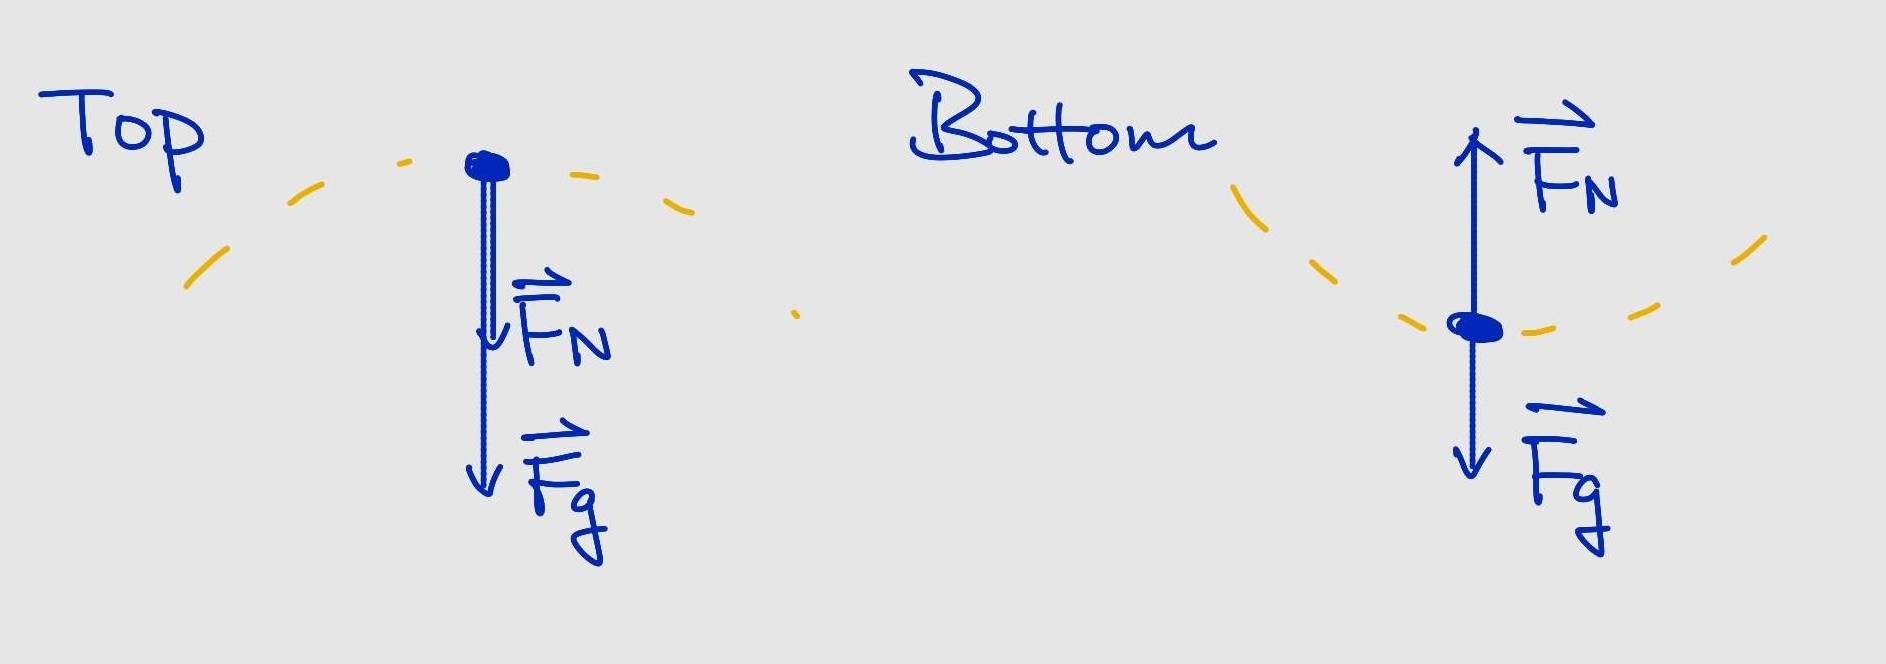
\includegraphics[scale=0.25]{fbdFn}
\end{center}

\textbf{Problem 1 part (2)}: At the bottom of the circular path, the plate is holding the cup, so the normal force is upward, and the gravitational force on the cup of water is downward. We want it to be able to maintain its circular motion, so we want a centripetal force (net force, the sum of normal force and gravitational force) to be pointing up, 
\begin{align*}
F_{\text{NET}} = \frac{mv^2}{R} = F_N - mg\,.
\end{align*}
The sign in front of each quantity is crucial. From here we can isolate $F_N$ and obtain
\begin{align*}
F_N = \frac{mv^2}{R} + mg\,.
\end{align*}

\textbf{Problem 1 Part (3)} At the top of the circular path, the cup is up-side-down, and the plate is preventing the cup to escape the circular path from above, so normal force in this case is pointing down. Gravitational force on the cup of water is again pointing down, and the centripetal force (sum of normal force and gravitational force) in this case should also point down in order to maintain circular motion.
\begin{align*}
F_{\text{NET}} = -\frac{mv^2}{R} = -F_N - mg\,.
\end{align*}
Again, the sign in front of each quantity is crucial. They are all negative because they are all pointing down. From here we get
\begin{align*}
F_N = \frac{mv^2}{R} - mg\,.
\end{align*}

\textbf{Problem 1 Part (4)}: At the top of the trajectory, if the spinning speed is too low, we expect the water cup will just fall down instead of going in a full circle (Imagine a car going through a vertical loop but with not enough speed, gravity is pulling too strong that the car will fall before going through the top of the loop). We notice that at the top of the circular path, both normal force and gravitational force point downwards, and they both contribute to the centripetal force (in the same way, same sign, but different magnitude). Speed $v$ of the cup of water is minimized when the magnitude of the centripetal force $mv^2/R$ is minimized, and thus is minimized when the sum of the magnitudes $F_N + mg$ is minimized. We are not able to change the mass $m$, nor the gravitational acceleration $g$, the radius $R$ is fixed, thus we can only change $F_N$ and make it zero to minimize the speed. 
\begin{align*}
-\frac{mv^2_{\min}}{R} = -F_N - mg = -mg \,,
\end{align*}
so we see
\begin{align*}
v_{\min} = \sqrt{gR}\,.
\end{align*}
This makes sense because normal force (at the top of the trajectory) is pulling the cup down, but gravitational force is already pulling it down to try to maintain the circular motion, so the speed-minimized situation occurs when normal force is zero. \\

\textbf{Problem 1 Part (5)}: We just need to plug in the numbers, 
\begin{align*}
&\text{Part (2): }F_N = \frac{mv^2}{R} + mg = 34.8\,\text{N}\,,\qquad
&\text{Part (3): }F_N = \frac{mv^2}{R} - mg = 15.2\,\text{N}\,,
\end{align*}
\begin{align*}
&\text{Part (4): }v_{\min} = \sqrt{gR} =3.13 \,\text{m/s}\,.
\end{align*}
The tangential speed that it is actually going is $5\,$m/s, which is faster than $v_{\min} = 3.13$ m/s found in part (4), so it is able to maintain its circular motion. \\

\textbf{Problem 2 Part (1)}: The tangential acceleration is simply $a_t = \alpha R$. \\

\textbf{Problem 2 Part (2)}: We have found the tangential acceleration as $a_t = \alpha R$, which is the rate of change of the tangential velocity, so after time $\Delta t$, 
\begin{align*}
v_t = v_0 + a_t\Delta t = v_0 + \alpha R\, \Delta t\,.
\end{align*}

\textbf{Problem 2 Part (3)}: For angular speed, we need to use the angular acceleration $\alpha$. Initially, the system has an angular speed $\omega_0 = v_0/R$, thus 
\begin{align*}
\omega = \omega_0 + \alpha \Delta t = \frac{v_0}{R} + \alpha \Delta t\,.
\end{align*}

\textbf{Problem 2 Part (4)}: The centripetal acceleration is 
\begin{align*}
a_c = \frac{v_t^2}{R}\,,
\end{align*}
where we have found the tangential velocity $v_t$ in part (2), so we write
\begin{align*}
a_c = \frac{(v_0+\alpha R\,\Delta t)^2}{R}\,.
\end{align*}

\textbf{Problem 2 Part (5)}: We just need to plug in numbers here, 
\begin{align*}
50 = \frac{(5+1\cdot 1\cdot \Delta t)^2}{1}
\end{align*}
we find $\Delta t = 2.07\,\text{s}$. At this time, the centripetal force is
\begin{align*}
F_c = ma_c = (1\,\text{kg})\cdot (50\,\text{m/s}^2) = 50 \,\text{N}\,.
\end{align*}

\end{document}


